\chapter{Examen de prueba: Autoevaluación del curso}
\section{Exercise 1}
We have a sequence 5241977 bases long. Table below shows the sequence statistics.

\begin{table}[htbp]
\centering
\begin{tabular}{l | l l l l l }
& overall & from A & from C & from G & from T \\ \hline
to A & 0.247 & 0.296 & 0.277 & 0.229 & 0.187 \\
to C & 0.253 & 0.223 & 0.231 & 0.323 & 0.235 \\
to G & 0.252 & 0.208 & 0.289 & 0.230 & 0.281 \\
to T & 0.247 & 0.273 & 0.202 & 0.218 & 0.298
\end{tabular}
\end{table}

How many TATA-box motifs (TATAAT) would you expect by chance according to a simple multinomial model?
$$ 0.247^6 \cdot 5241977 = 1190.36 \approx 1190 $$

And according to a Markov-chain model where the initial prob. is the same as overall one?
$$0.247 \cdot 0.187 \cdot 0.273 \cdot 0.187 \cdot 0.296 \cdot 0.273 \cdot 5241977 = 998.83 \approx 999 $$

\section{Exercise 2}
The following contains a python function that accepts a DNA sequence and returns the data structure AbsdiNucl\_freq containing the absolute frequencies of dinucleotides. 

\begin{lstlisting}
## Function to count absolute dinucleotide frequencies
def AbsdiNuclFrq(Seq):
	# Initializes a dictionary for all 16 potential dinucleotides
	AbsdiNucl_freq = {}
	for Base1 in ["A", "C", "G", "T"]:
		for Base2 in ["A", "C", "G", "T"]:
			AbsdiNucl_freq[Base1+Base2] = 0
	# count frequencies
	for pos in range(0, len(Seq) - 1):
		if Seq[pos:pos+2] in AbsdiNucl_freq.keys():
			AbsdiNucl_freq[Seq[pos:pos+2]] = AbsdiNucl_freq[Seq[pos:pos+2]]+1
	# Sequence length
	return(AbsdiNucl_freq) #return a identifier-null dict.
\end{lstlisting}

Which of the following expressions would you use to retrieve the frequency of the dinucleotide GC? \textbf{Since the frequencies are stored in a dictionary, we can just index by the dinucleotide we are interested in, so: AbsdiNucl\_freq["GC"]}

\section{Exercise 3}
The following figure shows several Dot-Matrix obtained from the alignment of different combinations of the indicated protein sequences or the indicated DNA sequences. Indicate which sequences were aligned in each case.
\begin{figure}[htbp]
\centering
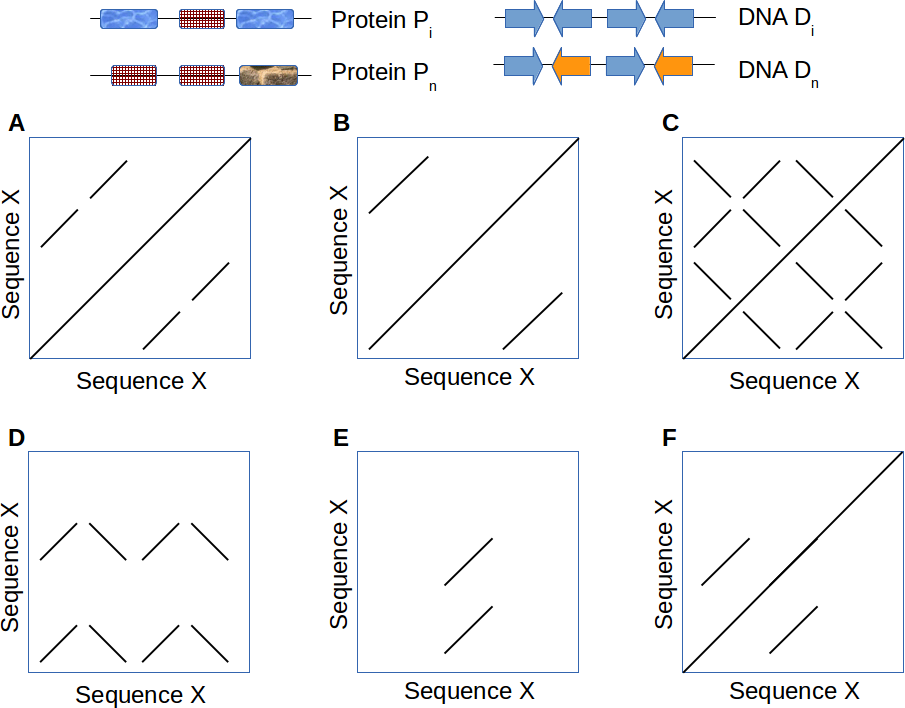
\includegraphics[width = 0.7\textwidth]{figs/exam-ex3.png}
\end{figure}

Trick: when a sequence is aligned with itself, there is a whole diagonal in the dot matrix.

\noindent
Dot-Matrix A: DNA Dn vs DNA Dn \\
Dot-Matrix B: Protein Pi vs Protein Pi \\
Dot-Matrix C: DNA Di vs DNA Di\\
Dot-Matrix D: DNA Di vs DNA Dn \\
Dot-Matrix E: Protein Pi vs Protein Pn \\
Dot-Matrix F: Protein Pn vs Protein Pn \\

\section{Exercise 4}
Indicate the optimal method to apply in the following situations:
\begin{enumerate}
\item Protein search against a database to identify similar proteins: \textbf{BLAST}
\item  You are interested in finding conserved domains within a set of given sequences: \textbf{Smith-Waterman - local alignment}
\item You need the best alignment between the whole extension of two proteins: \textbf{Needleman-Wunsch - global alignment}
\item Quick identification of repeated sequences between two chromosomes: \textbf{Dot-Matrix}
\end{enumerate}

\section{Exercise 5}
We performed a pairwise alignment between the human HRAS and the indicated \textit{C. elegans} proteins using BLAST(p) with default parameters and got the indicated scores. The figure shows the probability density (graphs on top) and cumulative probability (bottom graphs) for the BLAST score values for random alignments under these conditions (graphs on the right are just a zoom of the left graphs on the values 30 to 90). The red lines mark the position of problem scores. Indicate the probability of getting an alignment with an associated score equal or higher than these just by chance (choose the one that best describes it):

\begin{figure}[htbp]
\centering
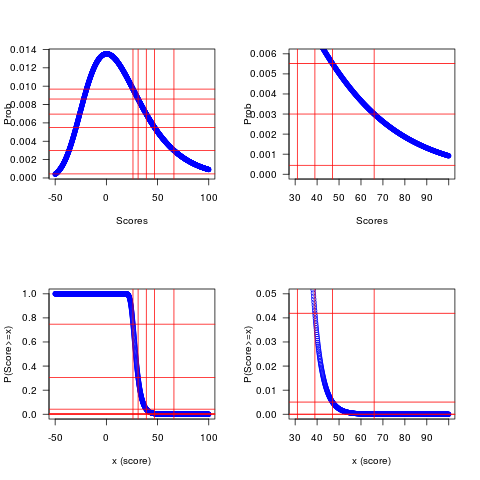
\includegraphics[width = 0.7\textwidth]{figs/exam-ex5.png}
\end{figure}

For this problem we have to use the cumulative probabilities (bottom graphs):
\begin{enumerate}
\item  KBRAS, score=120. p-value: \textbf{<0.001}
\item ARL2, score=66. p-value: \textbf{<0.001}
\item CKI1, score=47. p-value: \textbf{<0.01}
\item MED20, score=39. p-value: \textbf{<0.05}
\item ZK688, score=31. p-value: \textbf{>0.05}
\item RL15, score=26. p-value: \textbf{>0.05}
\end{enumerate}

\section{Exercise 6}
To generate the alignment between two sequences (of length m and n) using dynamic programing we follow these steps:
\begin{enumerate}
\item  Fill a m*n matrix with the scores resuting from: 
$$ Score = Max 
  \begin{cases}
    F(i-1, j-1) + s(x,y)\\ 
    F(i-1, j) - GapPenalty \\
    F(i, j-1) - GapPenalty
  \end{cases}
$$
  
\item  Reconstruct the alignment. Starting from bottom-right cell of the matrix generated in \#1 trace-back the pointers to the initial top-left cell.
\end{enumerate}

The pseudocode for this algorithm is depicted here:
\begin{figure}[htbp]
\centering
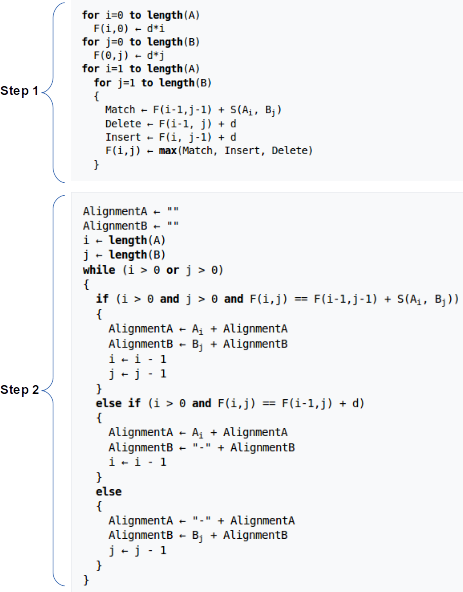
\includegraphics[width = 0.5\textwidth]{figs/exam-ex6.png}
\end{figure}

Are the pointers saved during the generation of the matrix (step 1)? \textbf{NO}

\section{Exercise 7}
Big-O notation is used to: \textbf{describe concisely the running time of an algorithm.}

\section{Exercise 8}
Match the following MSA with the simplest model that preserves most of the information in that alignment. keeping in mind that you can choose each model only once.
\begin{figure}[htbp]
\centering
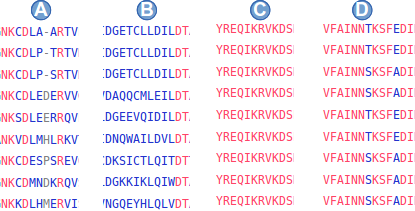
\includegraphics[width = 0.7\textwidth]{figs/exam-ex8.png}
\end{figure}

\noindent
Alignment A: \textbf{Hidden Markov Model (HMM)} \\
Alignment B: \textbf{Position Specific Scoring Matrix (profile) (PSSM)} \\
Alignment C: \textbf{Consensus sequence} \\
Alignment D: \textbf{Regular expression (pattern)}

\section{Exercise 9}
We have aligned several tyrosine protein kinases and found a conserved region corresponding to the active site of these enzymes. Here is the regular expression representing this alignment: [LIVMFYC]-{A}-[HY]-x-D-[LIVMFY]-[RSTAC]-{D}-{PF}-N-[LIVMFYC] 

\begin{figure}[htbp]
\centering
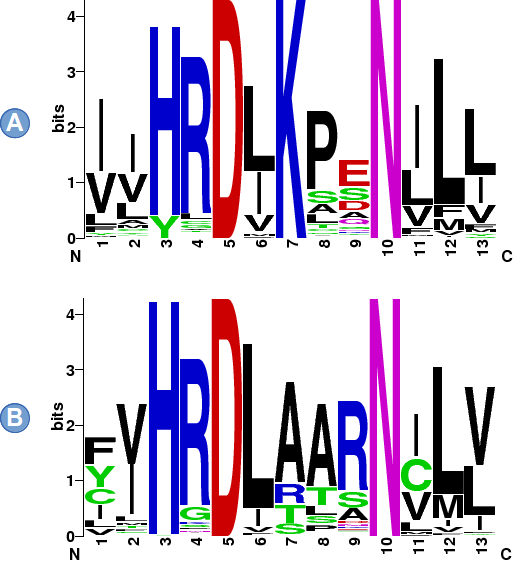
\includegraphics[width = 0.4\textwidth]{figs/exam-ex9.png}
\end{figure}

Which of the sequence logos in the figure represent this alignment? \textbf{B} \\
Which of the following positions shows the lowest information content in that alignment? \textbf{Position 1}

\section{Exercise 10}
Commonly used MSA programs: \textbf{use an heuristic approach composed of three steps: distance calculation, dendrogram tree generation, pairwise alignment based on tree topology.}

BLAST uses  an heuristic approach composed of three steps (construction of a word list from the sequences, identification of identical words (seeds), extension of seeds) for the search of a sequence within a database. 

Global and local alignments between two sequences  use an extension of dynamic programming to generate the alignment.